\section{Cartes d'identités}

\subsection{Python}

\begin{figure}[!ht]
	\center
	
\includegraphics[scale=0.4]{img/python.jpeg}
\end{figure}

\renewcommand{\labelitemi}{\textbullet}
\begin{itemize}
\item Généralités
	\begin{itemize}
	\item nom : Python
	\item version : 3.2 (sortie en 2011)
	\item date de création : 1990
	\item créateur : Guido van Rossum\\
	\end{itemize}
\item Paradigmes
	\begin{itemize}
	\item impératif
	\item orienté objet
	\item fonctionnel
	\item réflexif\\
	\end{itemize}
\item Typage
	\begin{itemize}
	\item fort
	\item dynamique
	\item implicite\\
	\end{itemize}
\item Divers
	\begin{itemize}
	\item turing-complétude : oui
	\item évaluation : stricte
	\item gestion de la mémoire : à la charge de l'implémentation\\
	\end{itemize}
\item Communauté
	\begin{itemize}
	\item popularité : langage populaire, parmi les 10 premiers
	\item implémentations : CPython, Jython, IronPython, PyPy\\
	\end{itemize}
\item Code
	\begin{itemize}
	\item code objet : principalement le code source mais du byte code peut aussi être généré
	\item Hello world! :
\begin{lstlisting}[language=python]
# Affichage standard
print("Hello world!")
\end{lstlisting}
	\end{itemize}
\end{itemize}

\newpage

\subsection{C++}

\begin{figure}[!ht]
	\center
	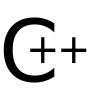
\includegraphics[scale=0.7]{img/cxx}
\end{figure}

\renewcommand{\labelitemi}{\textbullet}
\begin{itemize}
\item Généralités
	\begin{itemize}
	\item nom : C++
	\item version : 2008
	\item date de création : 1983
	\item créateur : Bjarne Stroustrup\\
	\end{itemize}
\item Paradigmes
	\begin{itemize}
	\item générique
	\item orienté objet
	\item procédural
	\item récursif
	\item …\\
	\end{itemize}
\item Typage
	\begin{itemize}
	\item faible
	\item statique
	\item explicite\\
	\end{itemize}
\item Divers
	\begin{itemize}
	\item turing-complétude : oui
	\item évaluation : stricte
	\item gestion de la mémoire : peut être gérée par l'utilisateur\\
	\end{itemize}
\item Communauté
	\begin{itemize}
	\item popularité : langage populaire, parmi les 5 premiers
	\item implémentations : g++, Borland C++ Compiler, Digital Mars, Visual C++, …\\
	\end{itemize}
\item Code
	\begin{itemize}
	\item code objet : code binaire, il s'agit d'un langage compilé
	\item Hello world! :
\begin{lstlisting}[language=c++]
#include <iostream> // Commentaire : utilisation de la sortie standard

int main(void)
{
    /* Commentaire : 'std::' sert a acceder a l'espace de noms std,
       dans lequel sont definies les variables cout et endl. */
    std::cout << "Hello world!" << std::endl;
    return 0;
}
\end{lstlisting}
	\end{itemize}
\end{itemize}

\newpage

\subsection{Prolog}

\renewcommand{\labelitemi}{\textbullet}
\begin{itemize}
\item Généralités
	\begin{itemize}
	\item nom : Prolog (acronyme de PROgrammation LOgique)
	\item version : 2000
	\item date de création : 1972
	\item créateurs : Alain Colmerauer, Philippe Roussel\\
	\end{itemize}
\item Paradigmes
	\begin{itemize}
	\item programmation logique
	\item récursif\\
	\end{itemize}
\item Typage : la qualification du typage du prolog n'a pas vraiment de sens puisqu'il n'existe pas réellement de variables. Cependant, en essayant d'extrapoler sur les mécanismes d'évaluation des valeurs il serait dynamique, fort et implicite\\
\item Divers
	\begin{itemize}
	\item turing-complétude : oui
	\item évaluation : paresseuse\\
	\end{itemize}
\item Communauté
	\begin{itemize}
	\item popularité : langage marginal ($> 30^{ème}$ place)
	\item implémentations : BProlog, GNUProlog, Poplog Prolog, P\#, …\\
	\end{itemize}
\item Code
	\begin{itemize}
	\item code objet : code binaire lorsque les performances comptent, parfois byte code en fonction de l'implémentation
	\item Hello world! :
\begin{lstlisting}[language=prolog]
?- write('Hello world!'), nl
Hello World!
true.
\end{lstlisting}
	\end{itemize}
\end{itemize}

\newpage

\subsection{Java}

\begin{figure}[!ht]
	\center
	
\includegraphics[scale=0.3]{img/java}
\end{figure}

\renewcommand{\labelitemi}{\textbullet}
\begin{itemize}
\item Généralités
	\begin{itemize}
	\item nom : Java
	\item version : 6.0 (sorti en 2006)
	\item date de création : 23 mai 1995
	\item créateur : Sun Microsystem\\
	\end{itemize}
\item Paradigmes
	\begin{itemize}
	\item générique
	\item orienté objet
	\item structuré
	\item impératif
	\item …\\
	\end{itemize}
\item Typage
	\begin{itemize}
	\item fort
	\item statique
	\item explicite\\
	\end{itemize}
\item Divers
	\begin{itemize}
	\item turing-complétude : oui
	\item évaluation : stricte
	\item gestion de la mémoire : gérée par l'implémentation\\
	\end{itemize}
\item Communauté
	\begin{itemize}
	\item popularité : langage populaire, parmi les 5 premiers
	\item implémentations : HotSpot, JamaicaVM, GIJ, OpenJDK, …\\
	\end{itemize}
\item Code
	\begin{itemize}
	\item code objet : byte code
	\item Hello world! :
\begin{lstlisting}[language=java]
// Hello World in Java
class HelloWorld
{
    static public void main(String args[])
    {
        System.out.println("Hello World!");
    }
}
\end{lstlisting}
	\end{itemize}
\end{itemize}

\newpage

\subsection{Brainfuck}

\renewcommand{\labelitemi}{\textbullet}
\begin{itemize}
\item Généralités
	\begin{itemize}
	\item nom : Brainfuck
	\item date de création : 1993
	\item créateur : Urban Müller\\
	\end{itemize}
\item Paradigmes
	\begin{itemize}
	\item à pile\\
	\end{itemize}
\item Typage (même si cela n'a pas beaucoup de sens)
	\begin{itemize}
	\item fort
	\item statique
	\item implicite\\
	\end{itemize}
\item Divers
	\begin{itemize}
	\item turing-complétude : oui
	\item gestion de la mémoire : gérée par l'implémentation\\
	\end{itemize}
\item Communauté
	\begin{itemize}
	\item popularité : langage exotique
	\item implémentations : il en existe une grande quantité vu que chacun peut en coder un facilement du fait de la simplicité du langage\\
	\end{itemize}
\item Code
	\begin{itemize}
	\item code objet : code source, langage interprété
	\item Hello world! :
\begin{lstlisting}
Hello world en Brainfuck
++++++++++[>+++++++>++++++++++>+++>+<<<<-]
>++.>+.+++++++..+++.>++.<<+++++++++++++++.
>.+++.------.--------.>+.>.
\end{lstlisting}
	\end{itemize}
\end{itemize}
